\section{チャーム・バリオン・スペクトロメータ}
図\ref{spectrometer}に、チャームバリオン・スペクトロメータの概要図を示す。
生成標的は$\SI{4}{\g / \cm^2}$の液体水素$(\rm{LH_2})$を用い、アクセプタンスが最大となるよう、スペクトロメータ磁石付近に設置する。
missing mass spectroscopyを用いる場合、ビーム粒子と散乱粒子を測定する必要がある。
そのため、チャーム・バリオン・スペクトロメータはビーム粒子測定用の検出器群と散乱粒子測定用の検出器群で構成されている。
ビーム粒子測定用の検出器群は、ビーム粒子を識別するためのリングイメージング・チェレンコフ検出器、ビーム粒子の通過タイミングを測定するためのビームタインミング検出器、
ビーム粒子の位置と角度を測定するためのシンチレーションファイバー検出器で構成される。
高運動量ビームを用いた固定標的実験の場合、$D^{*-}$からの崩壊粒子だけでなく、$Y_c^{*+}$からの崩壊粒子も前方へ放出される。
前方への崩壊粒子を効率よく測定するため、生成粒子測定には双極磁石システムを用いる。
ビーム粒子$(\pi^-)$の運動量が$\SI{20}{\GeV/c}$の場合、$D^{*-}$の崩壊粒子である$\bar{D^0}$から崩壊した$K^+$と$\pi^-$は2--16\space$\si{\GeV/c}$の運動量分布を持つ。
これらは、標的下流のシンチレーションファイバー検出器、ドリフト・チェンバー、閾値型チェレコフ検出器、リングイメージング・チェレンコフ検出器によって測定する。
また、$D^{*-}$からの低運動量の$\pi^-$と$Y_c^{*+}$からの崩壊粒子を広いアクセプタンスで測定するために、磁石内部にもタイミングカウンターと飛跡検出器を設置する。


\begin{figure}[htbp]
  \label{spectrometer}
  \centering
  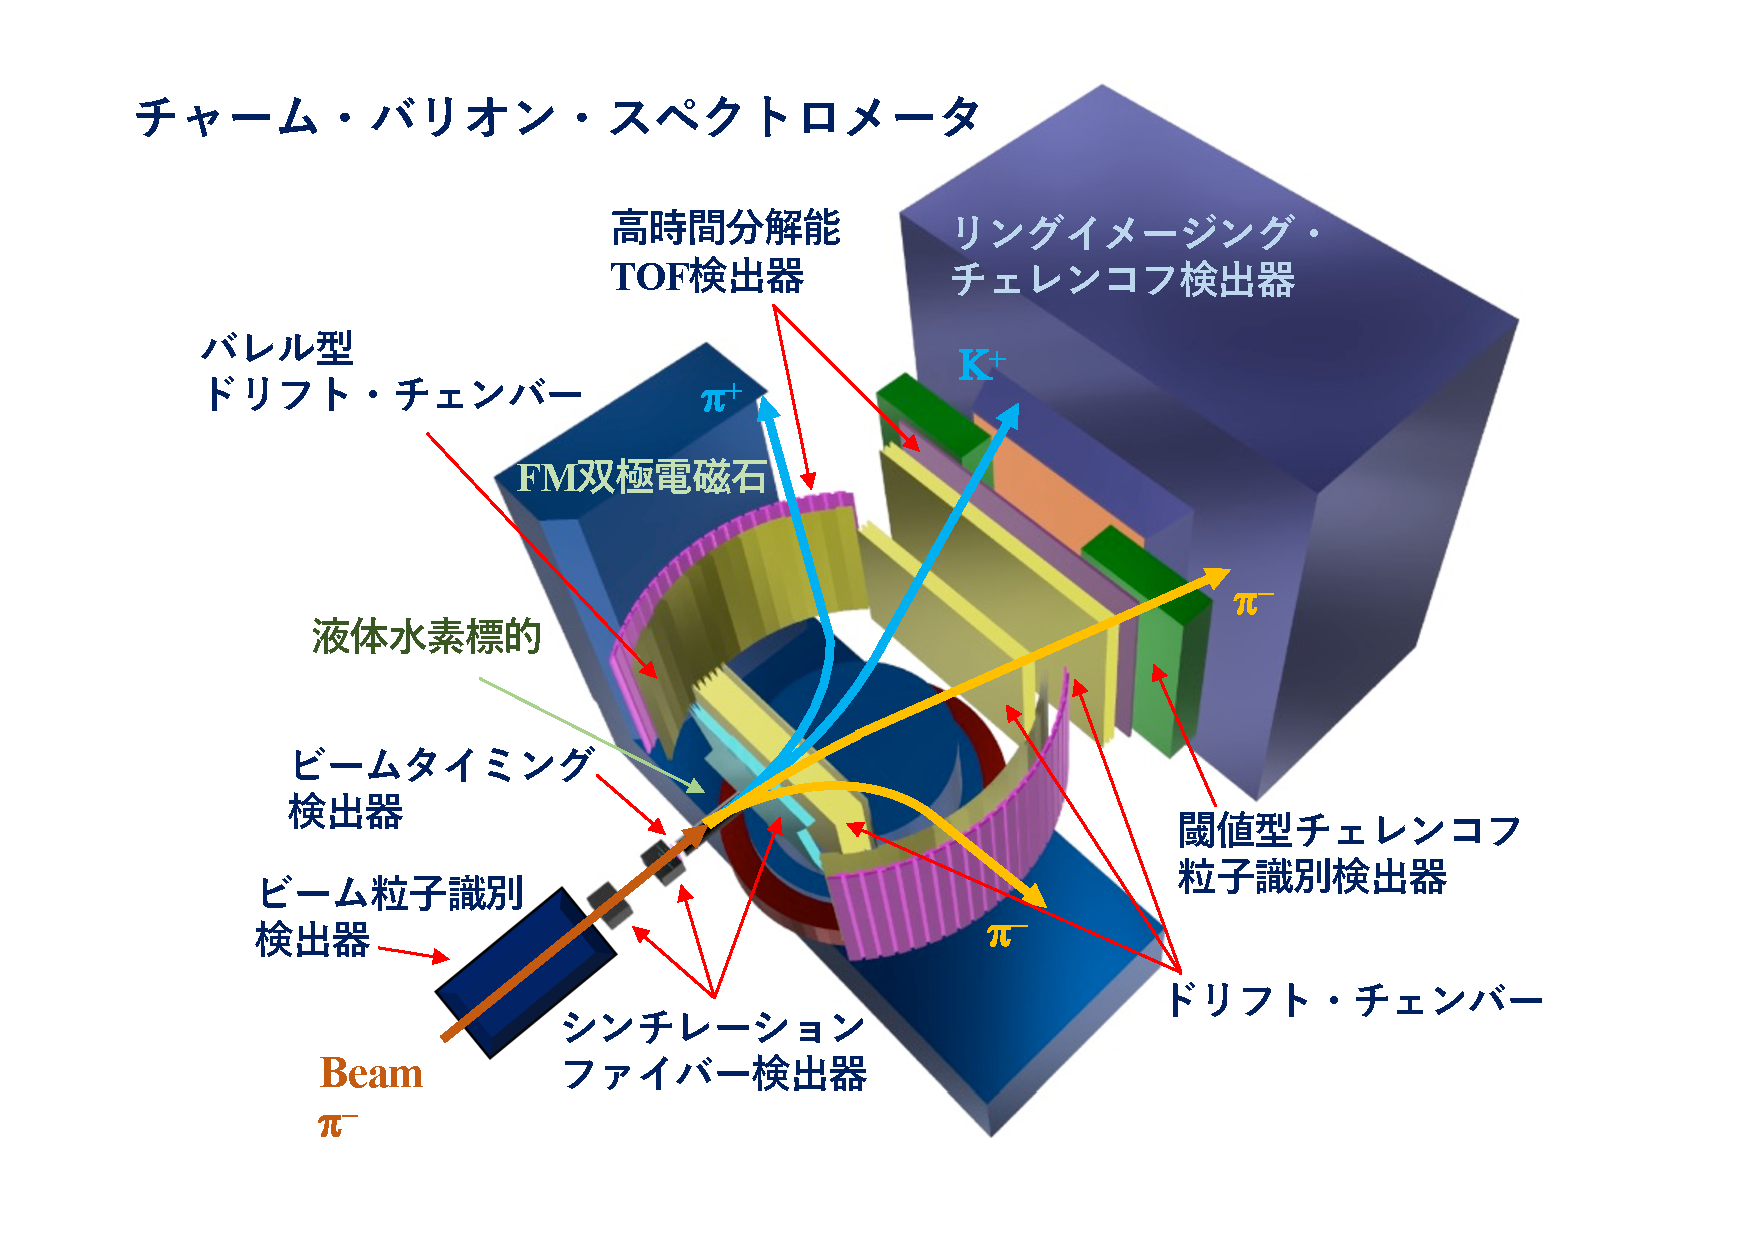
\includegraphics[width=15cm]{images/chapter1/spectrometer.pdf}
  \caption{チャーム・バリオン・スペクトロメータの概要図。ビーム粒子測定用検出器群と標的と反応して生成された粒子を測定する磁気スペクトロメータで構成される。}
\end{figure}